\documentclass[9pt,technote]{IEEEtran}

\usepackage[T1]{fontenc}
\usepackage[utf8]{inputenc}
\usepackage{amsmath}
\usepackage{cite}
\usepackage{newtxtext,newtxmath}
\usepackage{tablefootnote}
\usepackage{graphicx}
\usepackage{booktabs}
\usepackage{geometry}
\geometry{margin=0.55in}

\graphicspath{{./Figure/}}
\title{kNN Classifier}
\author{
	Gian Marco Balia\\
	Robotic Engineering - University of Genoa\\
	s4398275@studenti.unige.it
}

\begin{document}

\maketitle

\begin{abstract} 
The k-Nearest Neighbors (kNN) classifier is a supervised machine learning algorithm known for its simplicity and versatility, particularly effective in classification tasks. For instance, it is widely used in the medical field which highlights the importance of ontological approaches to optimize feature selection and enhance the robustness of kNN in complex contexts.

This report presents the implementation of kNN, emphasizing data preprocessing, relevant feature selection, and the optimization of the $k$ parameter. The algorithm was applied to a reference dataset to evaluate its performance in terms of accuracy and precision. The results demonstrate how the choice of $k$ significantly influences the trade-off between predictive accuracy and computational complexity.

\end{abstract}
\begin{IEEEkeywords}
 kNN Classifier, accuracy
\end{IEEEkeywords}

\section{Introduction}
In the rapidly evolving field of machine learning, the k-Nearest Neighbors (kNN) algorithm has emerged as a fundamental yet powerful tool for classification and regression tasks. Its intuitive approach—relying on proximity within the feature space to make predictions—makes kNN particularly attractive for applications where interpretability and simplicity are key. Despite its straightforward nature, the algorithm’s performance is deeply influenced by factors such as data preprocessing, feature selection, and the choice of the $k$ parameter, which determines the number of neighbors considered during classification.

One of the primary strengths of kNN lies in its versatility. It has been successfully applied in different fields, as image recognition, fraud detection, and medical diagnostics. A study \textit{"Fuzzy Decision Ontology for Melanoma Diagnosis Using kNN Classifier"} \cite{abbes2021FuzzyDecisionOntology} underscore the algorithm’s role in improving diagnostic accuracy through tailored feature selection strategies. However, kNN is not without limitations. It is sensitive to noise, computationally intensive for large datasets, and may struggle with imbalanced data.

There were implemented and evaluated the kNN algorithm focusing on its practical aspects, performance optimization, the impact of preprocessing techniques, the role of feature selection in reducing dimensionality, and the trade-offs involved in determining the optimal number of neighbors $k$.

By providing a comprehensive analysis of kNN's strengths, limitations, and potential improvements, this report aims to offer valuable insights for leveraging the algorithm effectively in real-world applications.
\section{Material and methods}

\subsection{Data processing}
This study is based on the analysis of a dataset describing various types of wines through their chemical characteristics and corresponding classifications. Specifically, the dataset is divided in two subsets: $wine.data$, which contains the chemical measurements associated with each wine sample (i.e., \textit{Alcohol}, \textit{Malic acid}, \textit{Ash}, \textit{Alcalinity of ash}, \textit{Magnesium}, \textit{Total phenols}, \textit{Flavanoids}, \textit{Nonflavanoid phenols}, \textit{Proanthocyanins}, \textit{Color intensity}, \textit{Hue}, \textit{OD280/OD315 of diluted wines}, \textit{Proline}), and $wine.target$, which identifies the specific class to which each wine in the analysis belongs.
Subsequently, both subsets were split and randomized to ensure accurate analysis. Specifically, the following subsets were generated:


\begin{itemize}
	\item $x_{train}$, containing $80\%$ of the data;
	\item  $x_{test}$, containing $20\%$ of the data;
	\item $y_{train}$, containing $80\%$ of the targets;
	\item $y_{test}$, containing $20\%$ of the targets.
\end{itemize}
In addition, prior to the analysis, it was necessary to normalize the obtained subsets. This step is crucial because the analysis involves calculating distances between different values. Given that the dataset contains variables with differing ranges of values, it is essential to scale the data to a uniform range to ensure that all features contribute equally to the computation of distances.
These subsets were then used for training and testing the kNN Classifier implemented in our study.
\subsection{kNN Classifier}
The implementation of k-Nearest Neighbors (kNN) algorithm is based on computing of normalized linear distance between the points of the training set and the evaluated test's point.
After computing the distance, the algorithm predicted the class to which points belong based on the number of neighbors $k$.

\subsection{Model evaluation}
The model was evaluated computing its accuracy in relation to the specific $k$ parameter considered during the analysis and model training. As mentioned earlier, the $k$ parameter represents the number of nearest neighbors taken into account for classifying a new data point, determining how many points in the training dataset are chosen to decide the class of a sample. The results obtained, specifically the model's accuracy for each value of $k$, are displayed in Figure \ref{fig::accuracy}.
Another parameters used to evaluate the model are: the \textit{error rate}, which represent the percentage of incorrect predictions; the \textit{precision} that characterize the proportion of true positives (correctly classified instances) among all positive predictions made by the classifier; the \textit{recall} which is the proportion of true positives among all actual positive instances; the \textit{F1 Score} that represent the harmonic mean of precision and recall, providing a balanced measure of both.
The last three parameters are obtained with a \textit{confusion matrix}. A \textit{confusion matrix} is a table used to evaluate the performance of a classification model by comparing its predictions against the actual outcomes. It provides a detailed breakdown of prediction accuracy across different classes, offering insight into the model’s strengths and areas for improvement. The confusion matrix is structured as follows:
\begin{equation*}
	\text{C}=\begin{pmatrix}
		\text{TP} & \text{FP} \\
		\text{FN} & \text{TN}
	\end{pmatrix}
\end{equation*}
where the \textit{true positives} (TP) are the cases where the model correctly predicted the positive class; the \textit{true negatives} (TN) are the cases where the model correctly predicted the negative class; the \textit{false positives} (FP) are the cases where the model incorrectly predicted the positive class (Type I error); and the \textit{false negatives} (FN) is the cases where the model incorrectly predicted the negative class (Type II error).


\begin{table}[h!]
    \centering
    \caption{Class 0 Statistics over all k values}
    \begin{tabular}{@{}lrrrrr@{}}
        \toprule
        Metric    & Mean     & Median   & AAD       & 1st Quantile & 3rd Quantile \\
        \midrule
        Precision & 0.987879 & 1        & 0.0198347 & 1           & 1            \\
        Recall    & 0.991736 & 1        & 0.0135237 & 1           & 1            \\
        F1 Score  & 0.989797 & 1        & 0.0129861 & 0.971941    & 1            \\
        \bottomrule
    \end{tabular}
\end{table}

\begin{figure}[h]
	\centering
	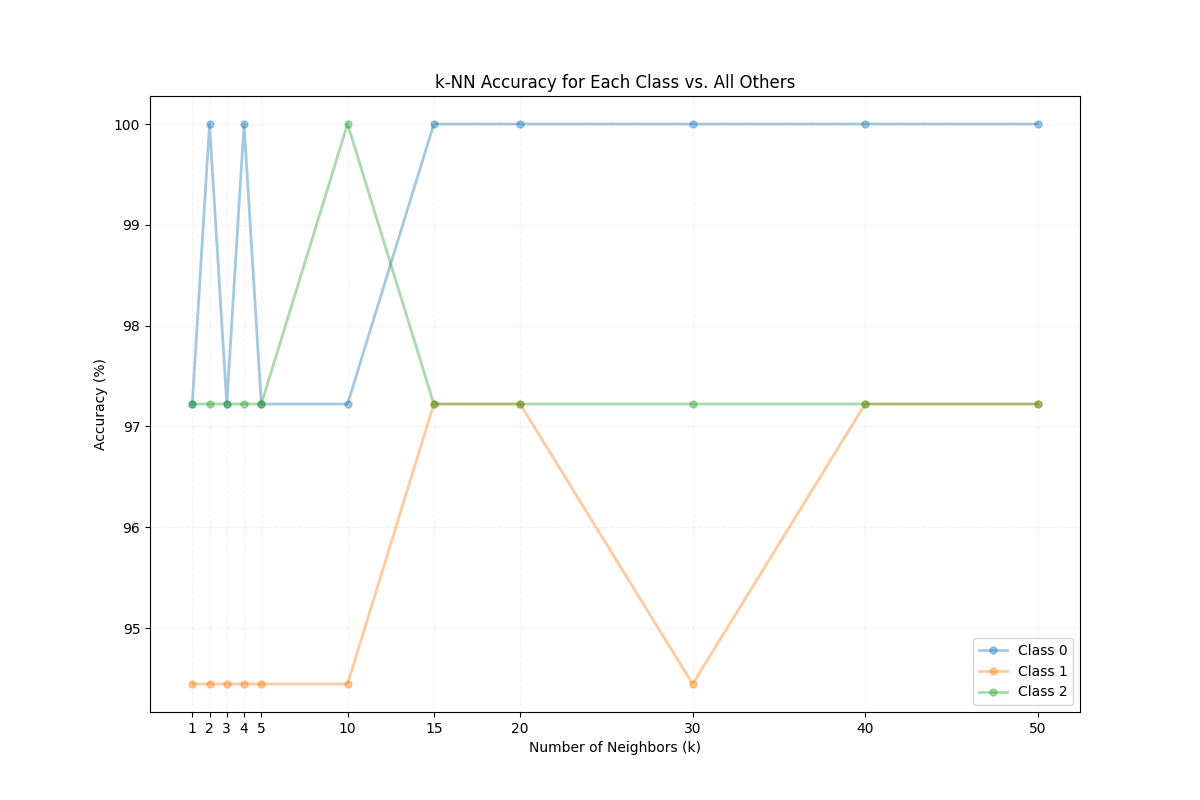
\includegraphics[width=0.5\textwidth]{accuracy.png}
	\caption{Relationship between the number of neighbors $k$ and the classification accuracy across all classes for the kNN classifier.}
	\label{fig::accuracy}
\end{figure}

\section{Results and Conclusion}
The parameter $k$ determines how many neighbors are considered to make the classification. The value of $k$ has a significant impact on the model's performance. If $k$ is too small, the algorithm can be sensitive to noise in the data and may lead to overfitting, where the model fits too closely to the training data. On the other hand, if $k$ is too large, it can reduce the model's ability to capture local variations in the data, resulting in under-fitting, where the model fails to adequately represent the complexities of the dataset. As shown in Figure \ref{fig::accuracy}, choosing the optimal value of $k$ is crucial to balance accuracy and computational complexity.
In Figure \ref{fig::accuracy}, are highlighted the two optimums number of neighbors $k$ three and four.
% TODO Highlight that the error rate in the first class i very high (100%)
\bibliographystyle{IEEEtranS}
\bibliography{Bib.bib}

\end{document}